\documentclass{beamer}
\usepackage{amssymb}% http://ctan.org/pkg/amssymb
\usepackage{pifont}% http://ctan.org/pkg/pifont
\usepackage{subcaption}
\usepackage{comment}
\usepackage{csvsimple, booktabs}
\logo{
\includegraphics[width=15mm,scale=0.2]{uib_01.png}}
\beamertemplatenavigationsymbolsempty
\usetheme{PaloAlto}
%\usecolortheme{wolverine}
%\setbeamertemplate{headline}{} % not showing on top
\setbeamertemplate{footline}[page number]

%Information to be included in the title page:
\title{A simple detector for crowd counting using OpenCV and Python}
\author{Martí Gelabert Gómez}
\institute{University of the Balearic Islands}
\date{\today}

\AtBeginSection[]{
  \begin{frame}
  \vfill
  \centering
  \begin{beamercolorbox}[sep=8pt,center,shadow=true,rounded=true]{title}
    \usebeamerfont{title}\insertsectionhead\par%
  \end{beamercolorbox}
  \vfill
  \end{frame}
}

\begin{document}

\frame{\titlepage}

\begin{frame}

    \frametitle{Objective}
    \centering
    Create a crowd counting algorithm.\newline \pause

    We can implement it as we want!\newline \pause

    Now what? Where do we have to start?

\end{frame}


\begin{frame}
    \frametitle{Where do we start}
    First, we need to label our images and establish some kind of criteria to decide to label it or not. 
     
\end{frame}


\begin{frame}
    \frametitle{Where do we start}
    Now, we need a way for detecting people:
    \begin{itemize}
        \item<2-> Gabor filtering  \pause {\color{red} \ding{55}}
        \item<3-> Edge detector  \pause {\color{red} \ding{55}}
        \item<4-> Applying derivatives \pause {\color{red} \ding{55}}
        \item<5-> Background removal  {\color{green} \checkmark}
    \end{itemize}
     
\end{frame}

%\frame{\tableofcontents}

\begin{comment}
    \section*{Procedure}
\begin{frame}
\frametitle{Procedure}
\begin{enumerate}
    \item Import images as black and white.
    \item Apply Adaptative Histogram equalization to the images.
    \item Substract the background to the images using the image with the background.
    \item Apply an erosion algorithm to obtain small highlighted areas.
    \item Apply a thresholding algorithm to binarize the image.
    \item Apply a dilation operation into the binarized images to expand the whites.
    \item Use a contour algorithm to extract the diferent regions containing persons.
    \item Obtain the bounding boxes from these regions.
    \item Count them and compare the number of detections to the real cuantity.
\end{enumerate}\end{frame}
\end{comment}



\section{Background Removal}
    \begin{frame}
        \frametitle{Background Removal}
        \begin{figure}
            \centering
            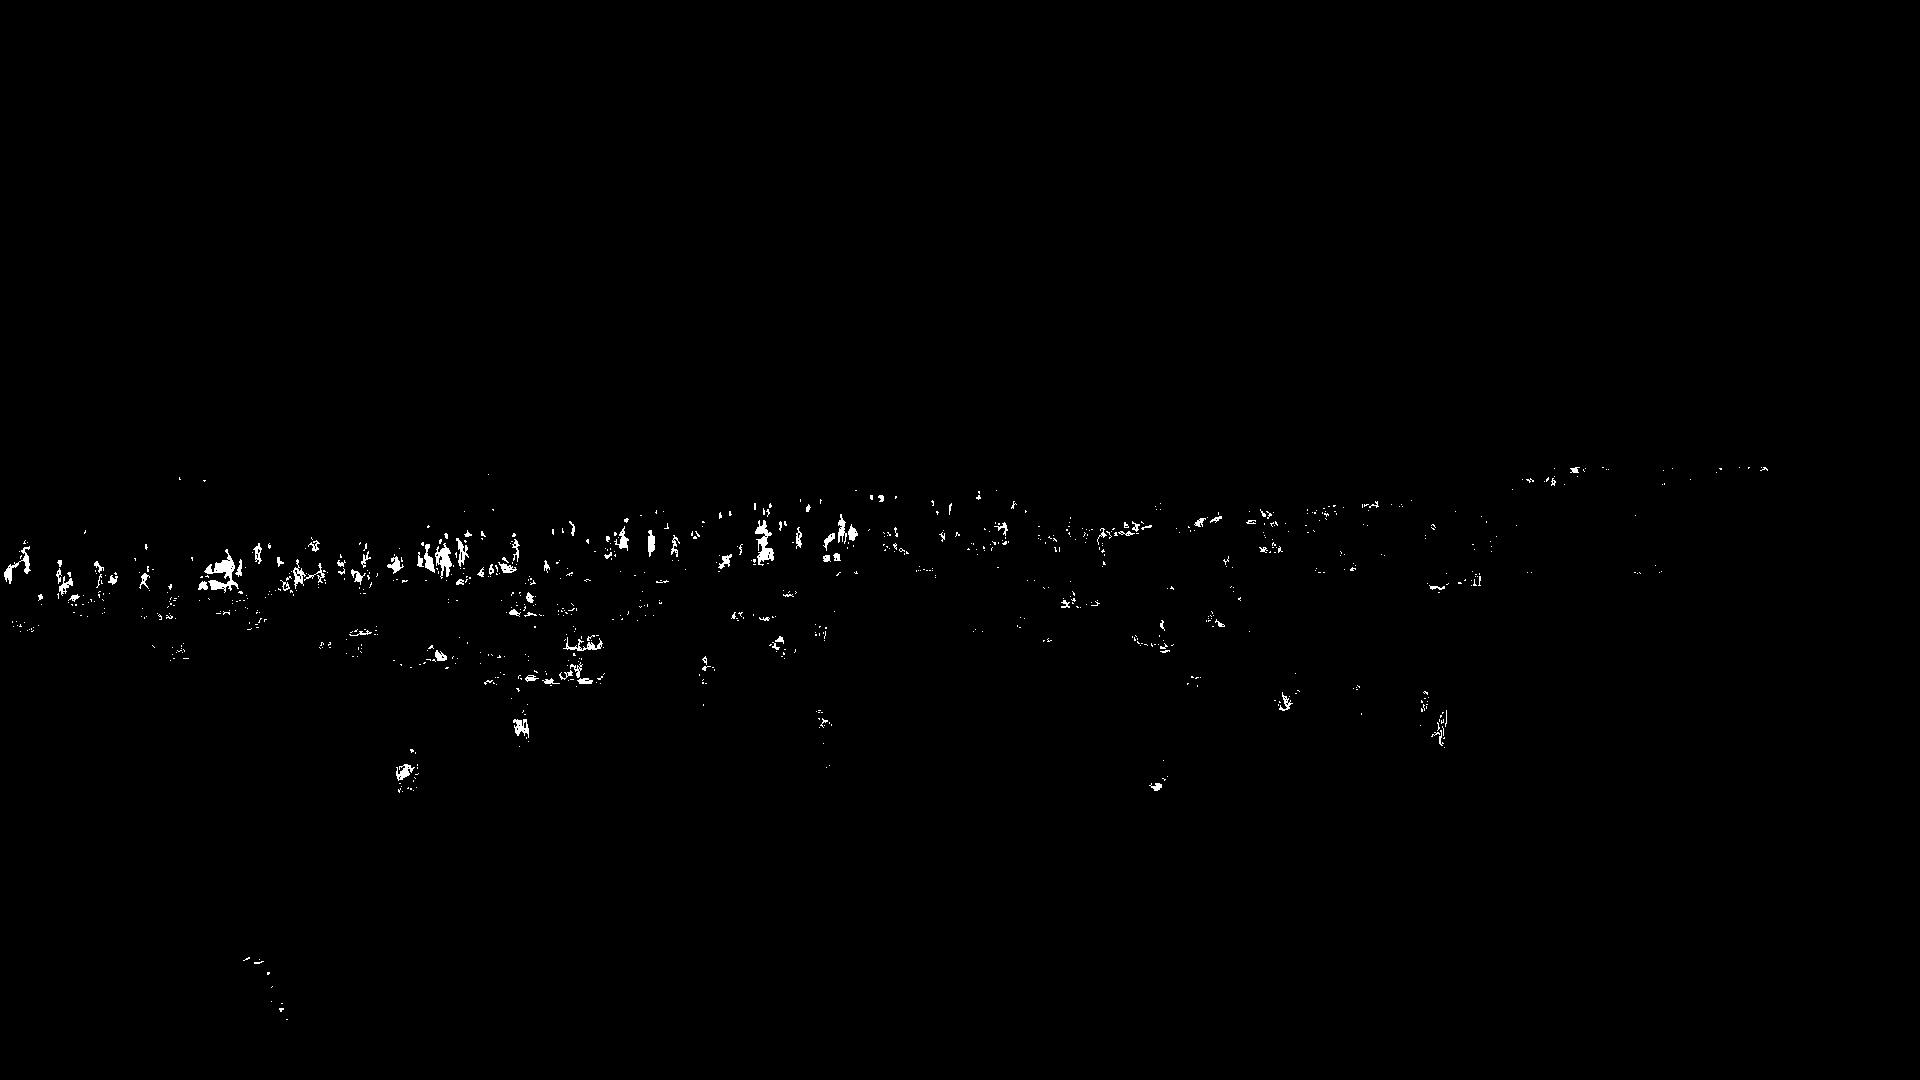
\includegraphics[width=\textwidth]{../gen/bin/1660320000.jpg}
        \end{figure}
    \end{frame}

\begin{frame}
        We need to do something with the \textbf{illumination} of the images and improve the \textbf{contrast}.
\end{frame}
\subsection*{CLAHE}

\begin{comment}
    \begin{frame}
        \frametitle{CLAHE}
        We need to do something with the illumination of the images.
        \begin{columns}[c]
            % create the column with the first image, that occupies
            % half of the slide
                \begin{column}{.5\textwidth}
                \begin{figure}
                    \centering
                    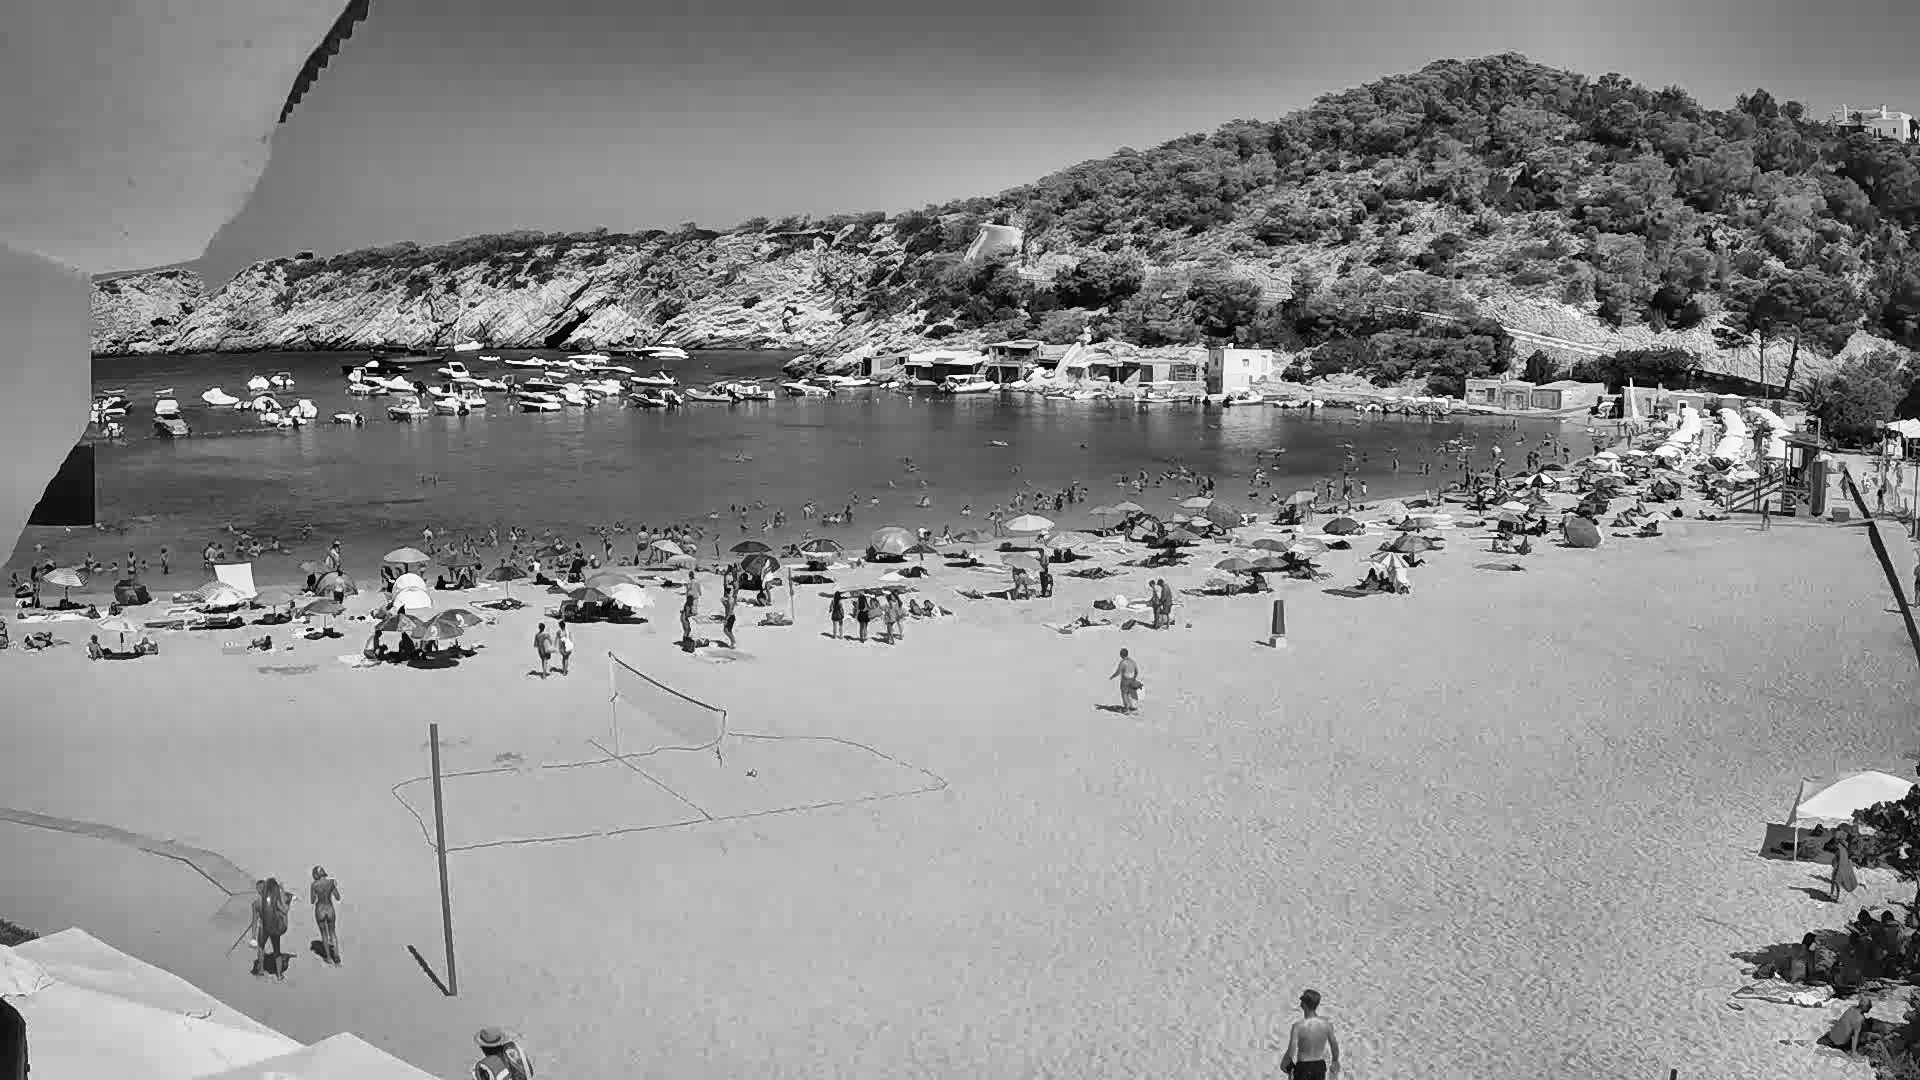
\includegraphics[width=\textwidth]{../gen/equ/1660298400.jpg}
                    
                \end{figure}      
                \end{column}
            % create the column with the second image, that also
            % occupies half of the slide
                \begin{column}{.5\textwidth}
                \begin{figure}
                    \centering
                    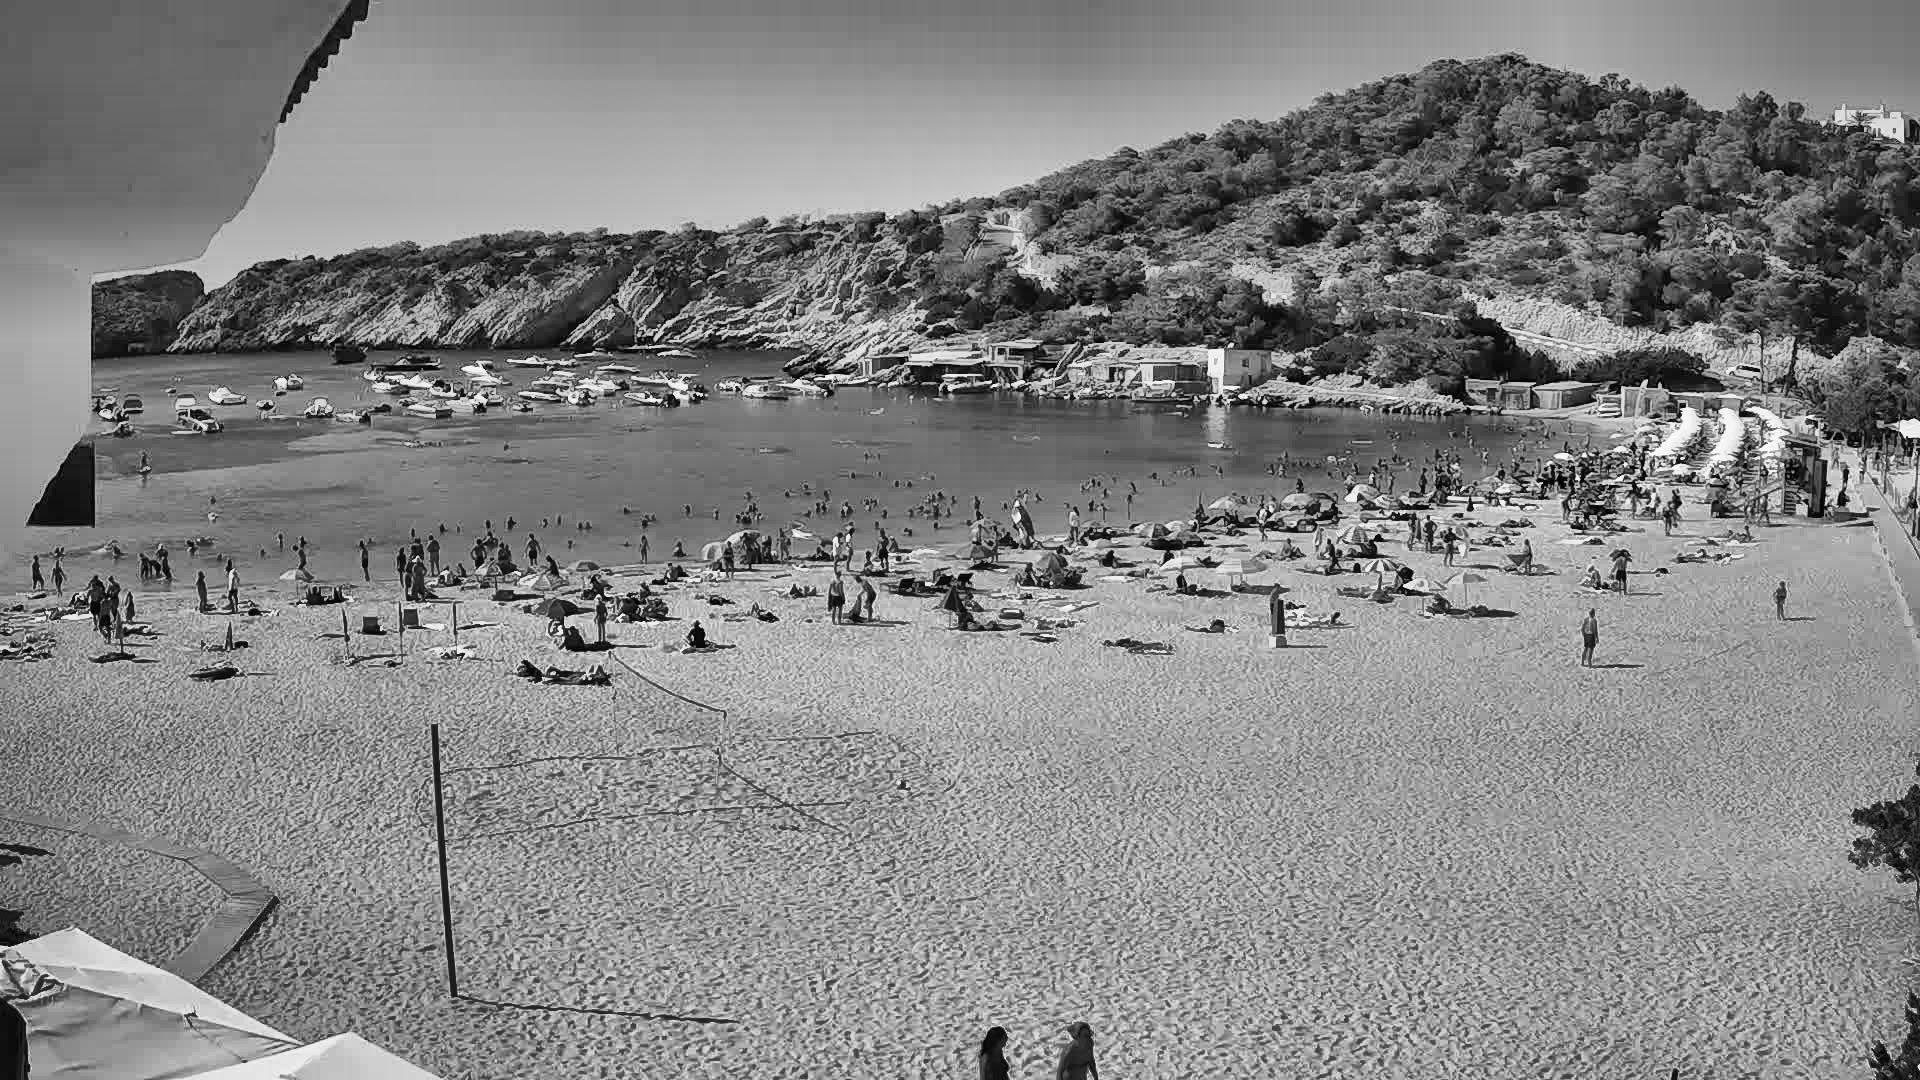
\includegraphics[width=\textwidth]{../gen/equ/1660316400.jpg}                 
                \end{figure}
                \end{column}
            \end{columns}
    \end{frame}
\end{comment}

\begin{frame}
    \frametitle{CLAHE}
    \centering
    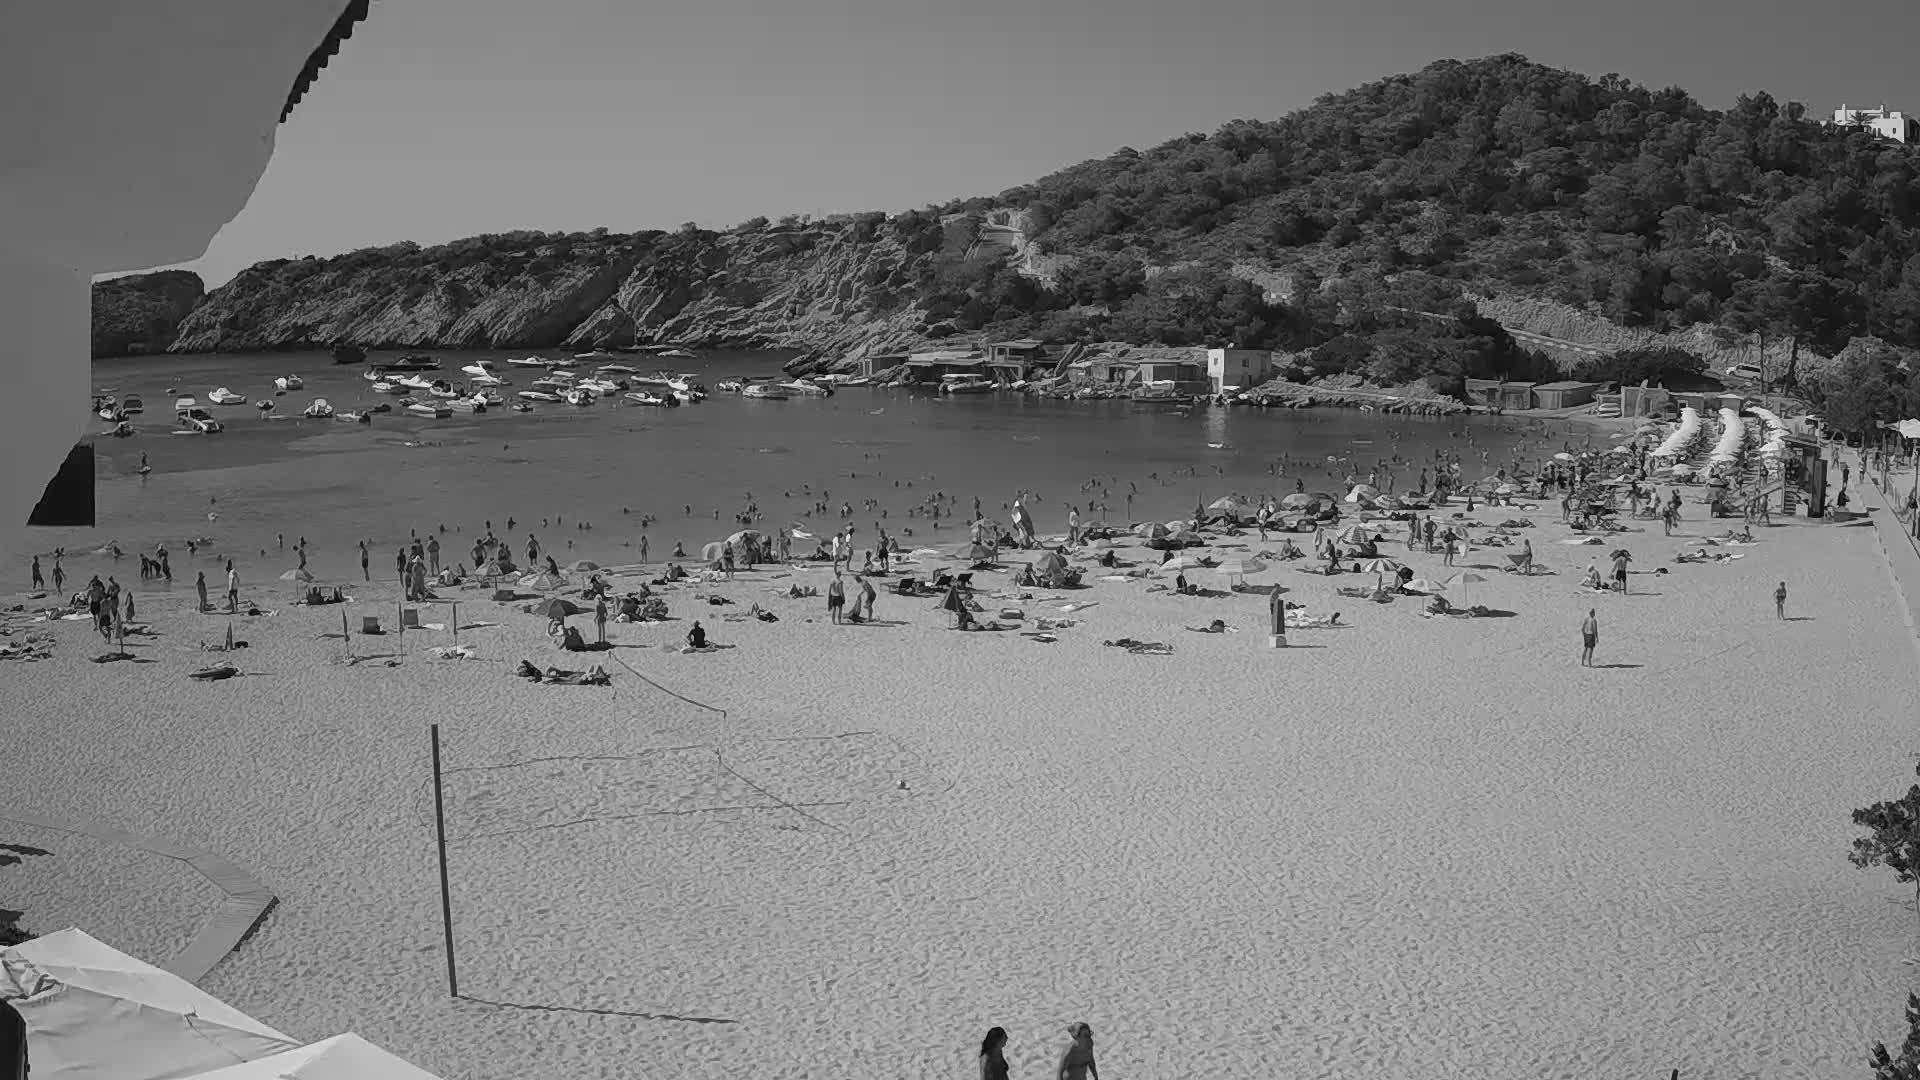
\includegraphics[width=\textwidth]{../gen/gray/1660316400.jpg}
  
\end{frame}

\begin{frame}
    \centering
    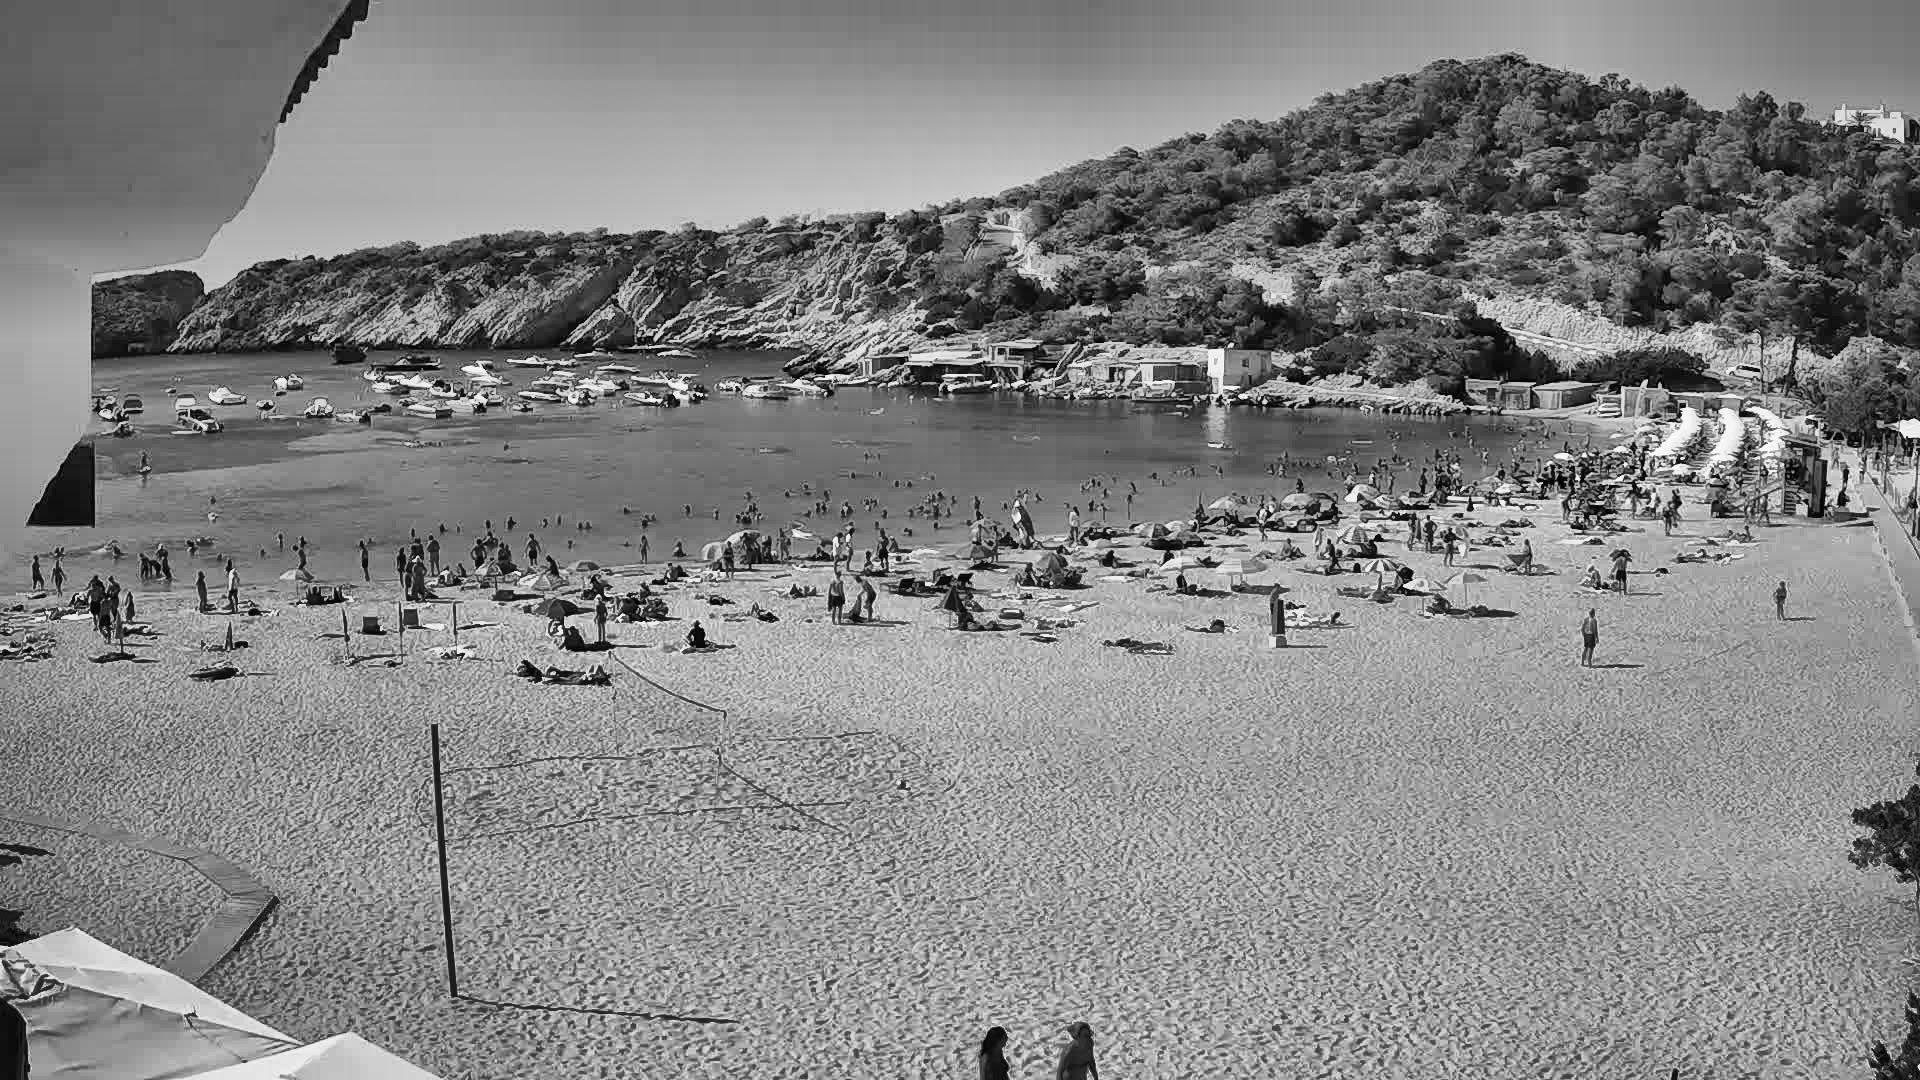
\includegraphics[width=\textwidth]{../gen/equ/1660316400.jpg} 
\end{frame}

\subsection*{Background Image}
\begin{frame}
    \frametitle{Background Image}

    \begin{figure}
        \centering
        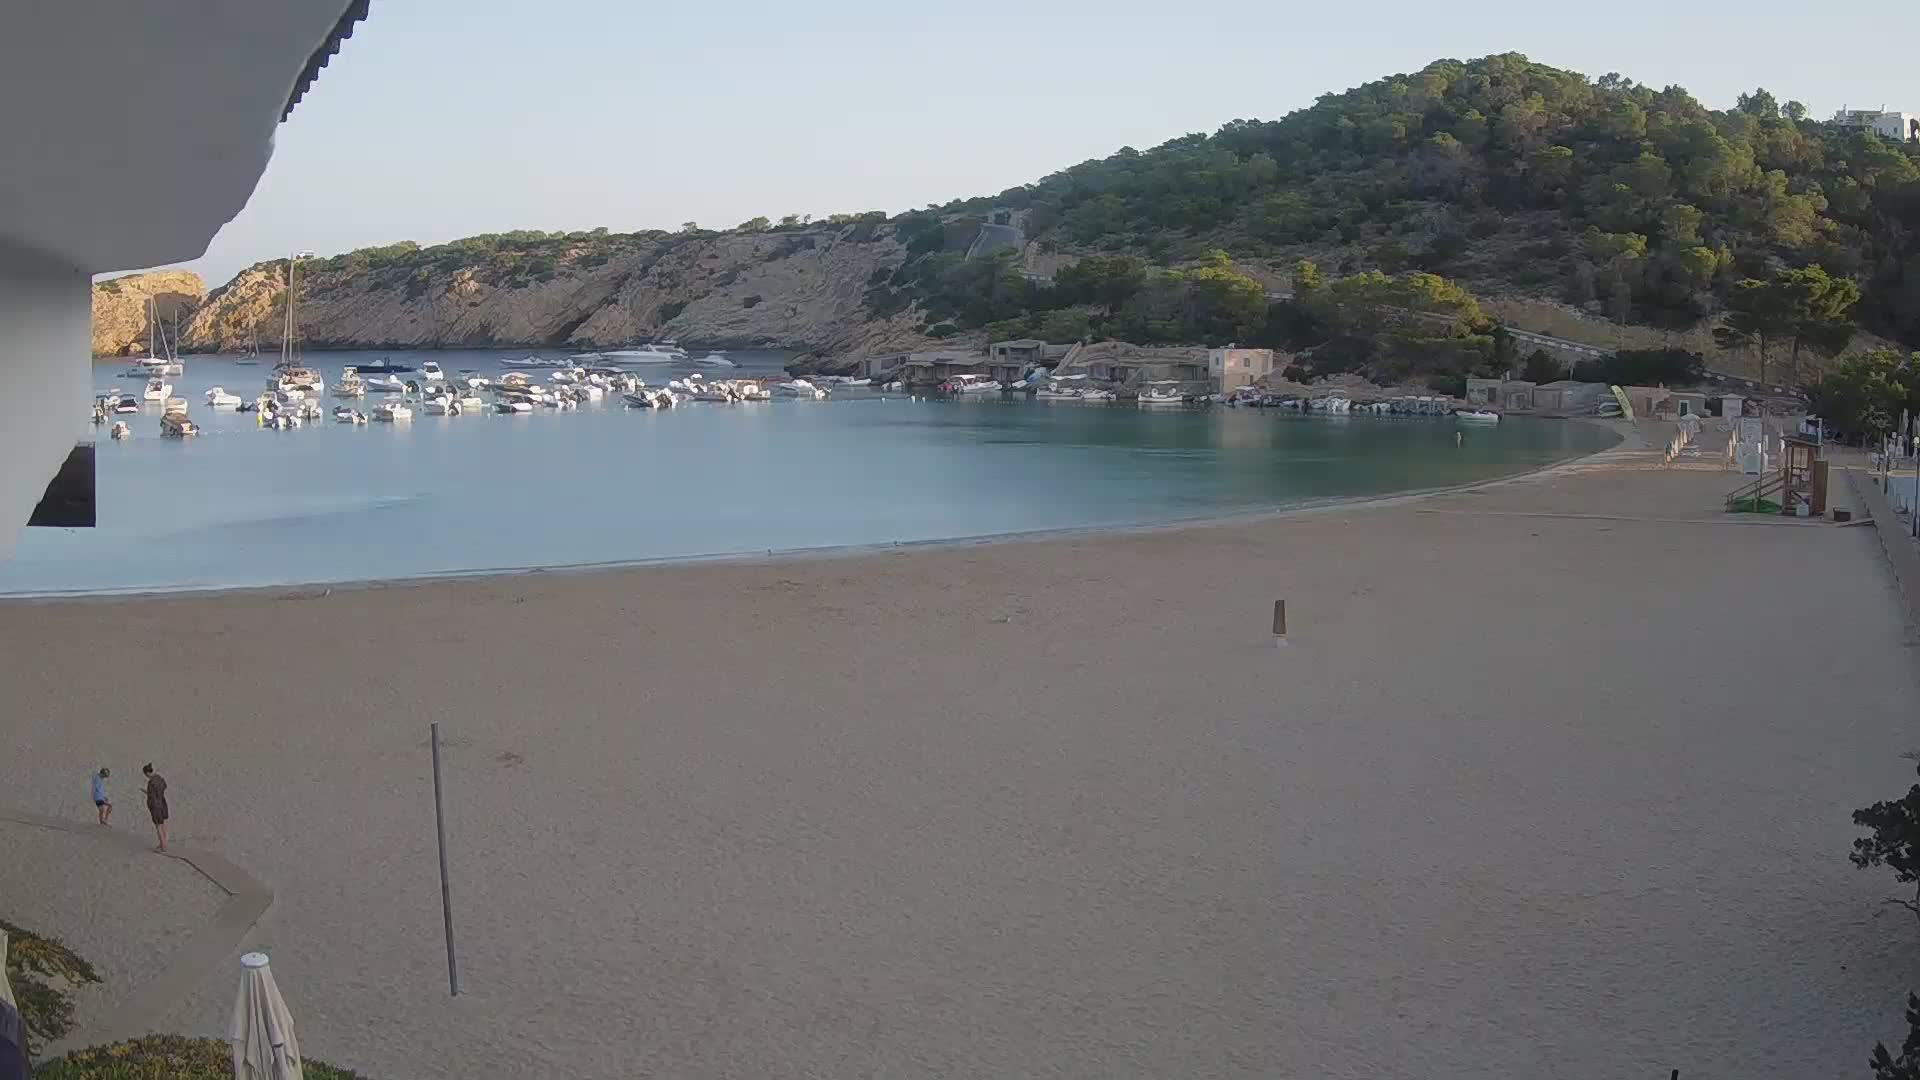
\includegraphics[width=\textwidth]{../Gelabert/1660284000.jpg}
    \end{figure}

\end{frame}

\begin{frame}
    \frametitle{Average image \ding{55}}

    \begin{figure}
        \centering
        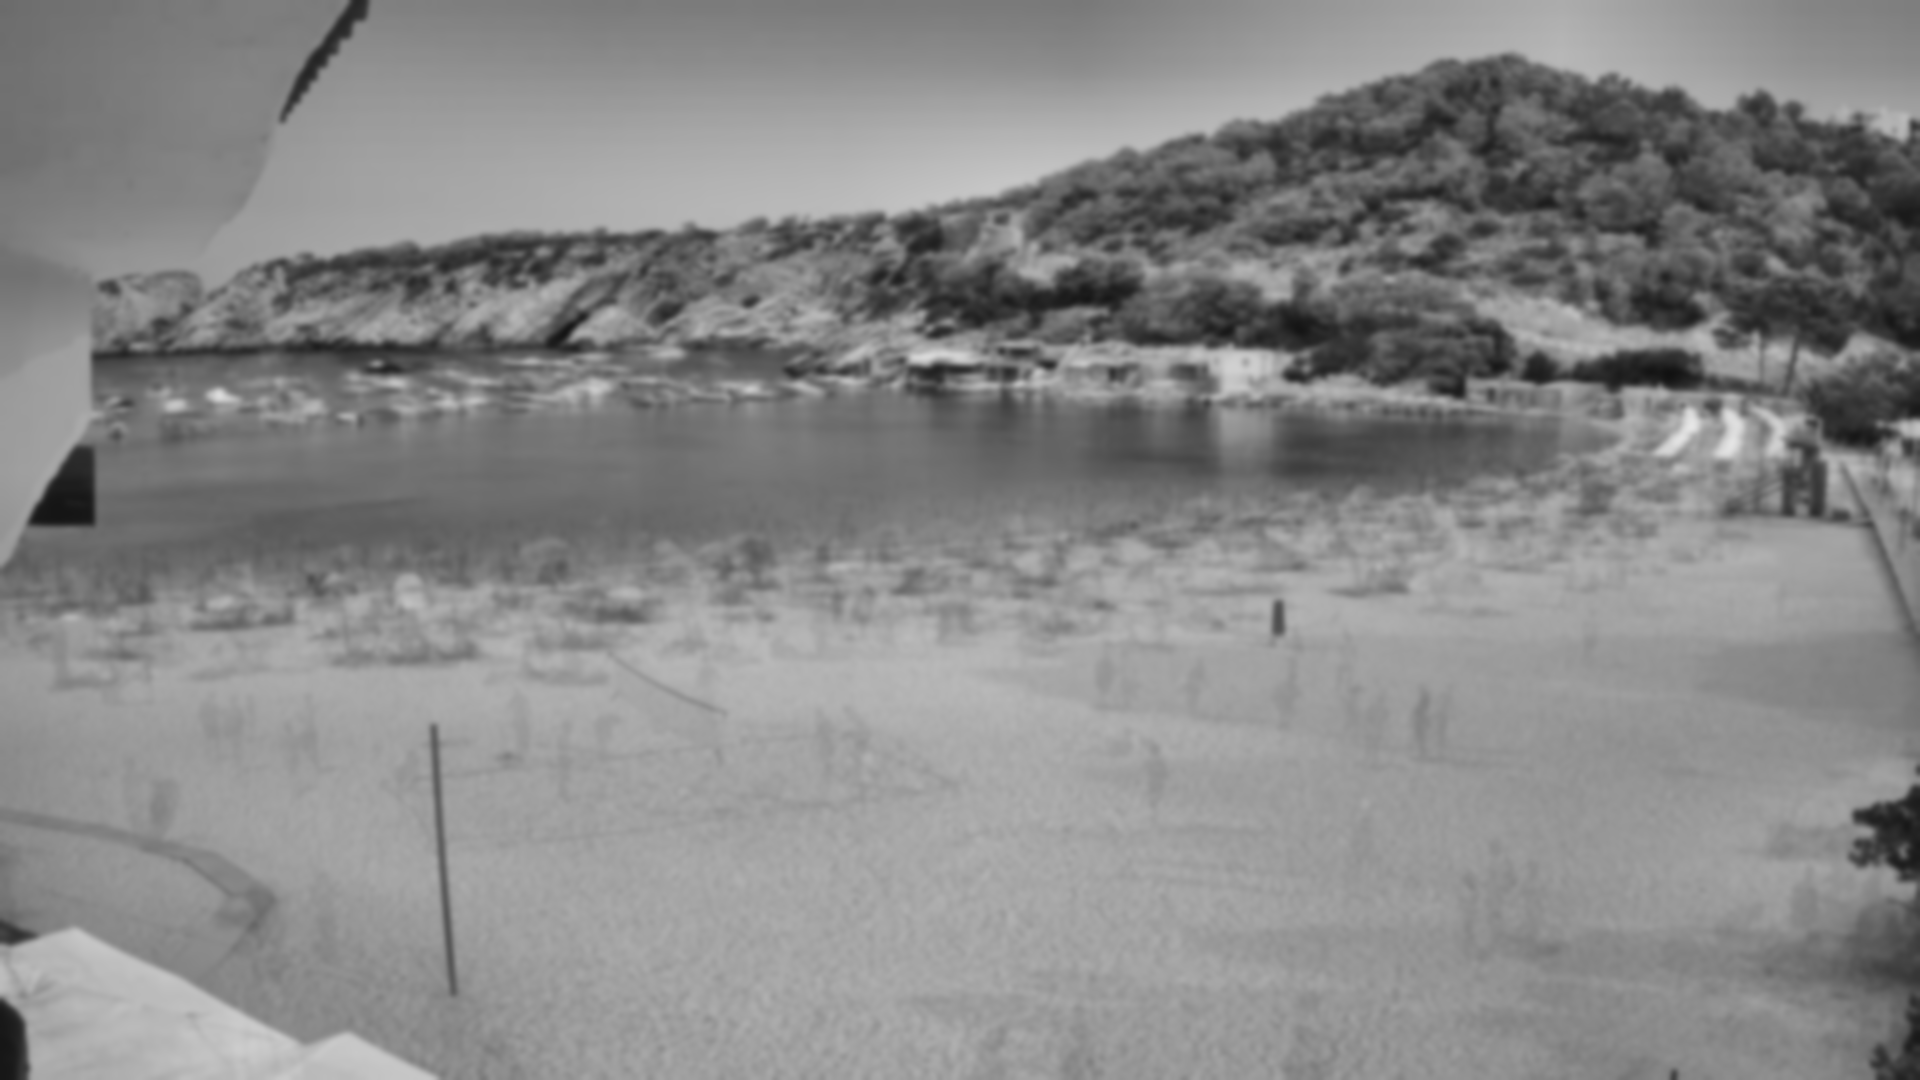
\includegraphics[width=\textwidth]{../gen/avg.png}
    \end{figure}
    
\end{frame}

\subsection*{Gaussian Blur}
\begin{frame}
    \frametitle{Gaussian Blur}
    \begin{figure}
        \centering
        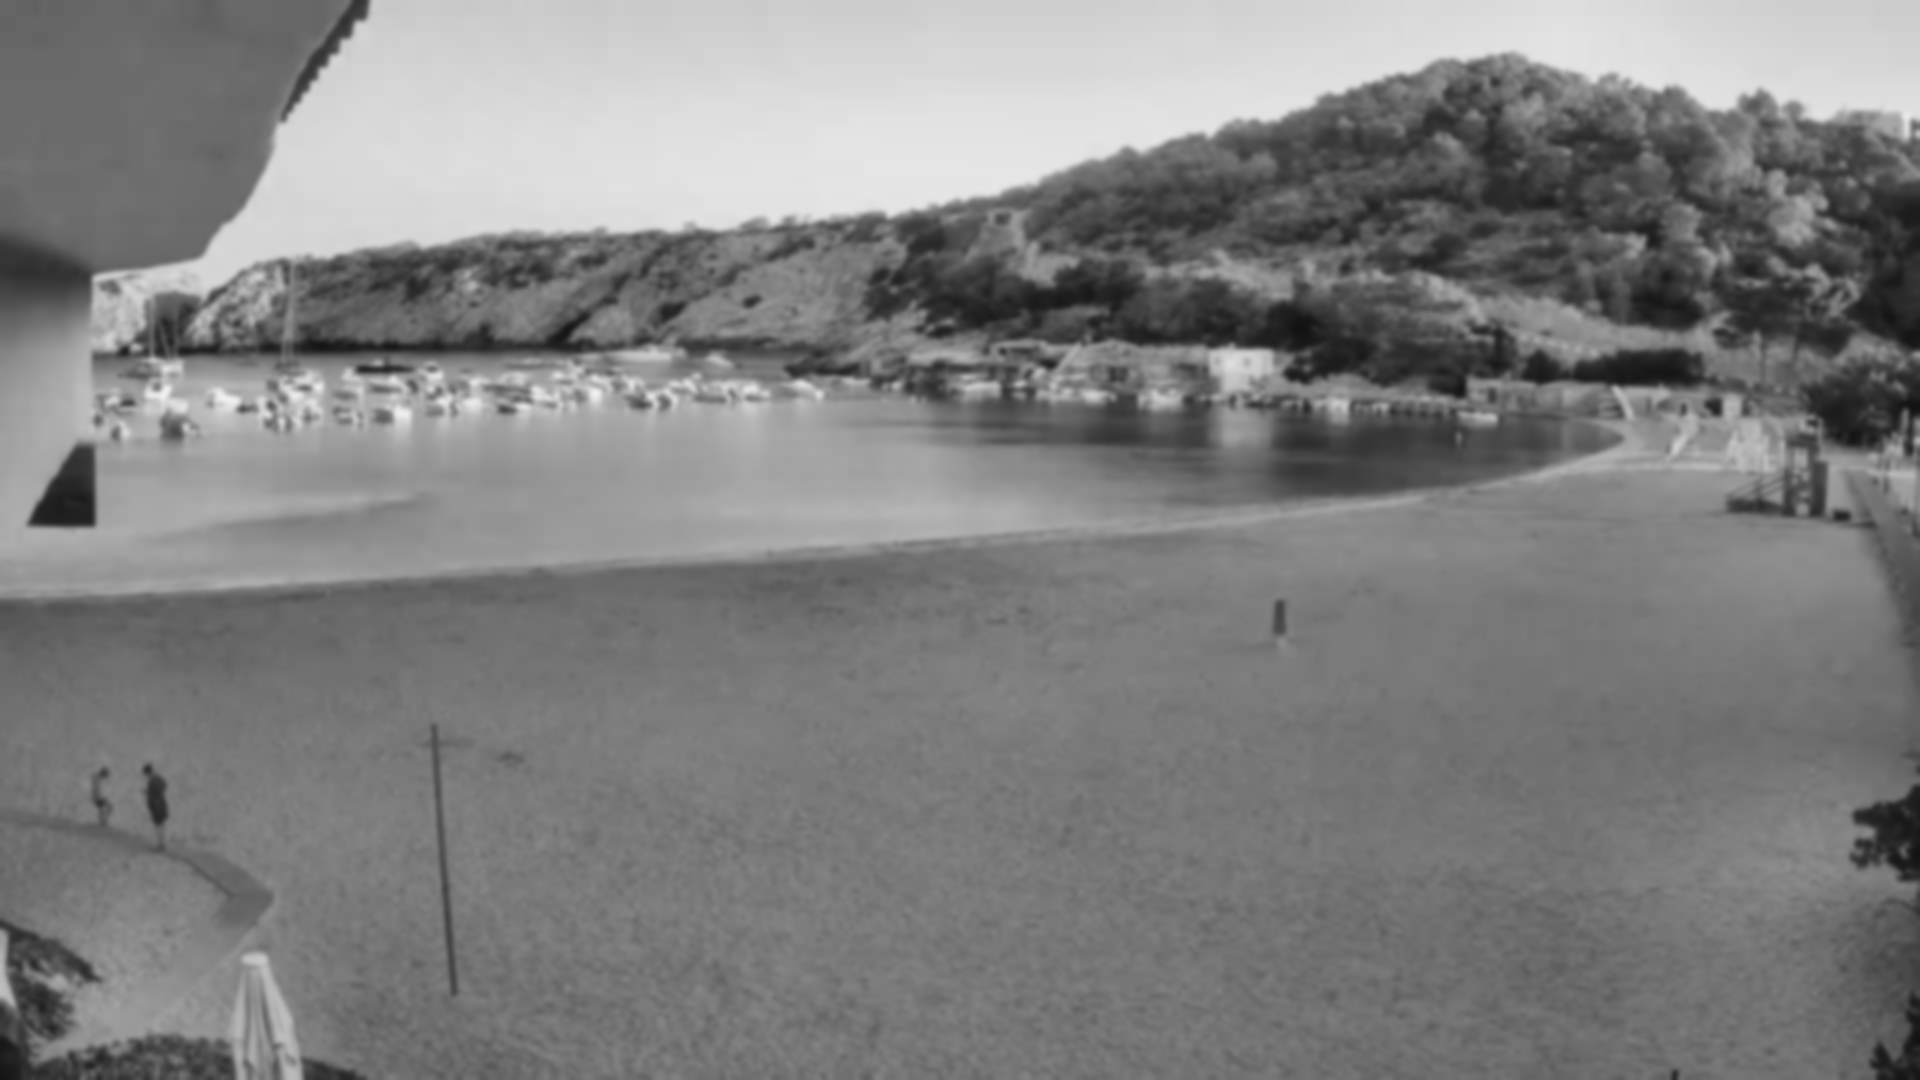
\includegraphics[width=\textwidth]{../gen/blur.png}
    \end{figure}

\end{frame}

\subsection*{Substraction}
\begin{frame}
    \frametitle{Substraction}
    \begin{figure}
        \centering
        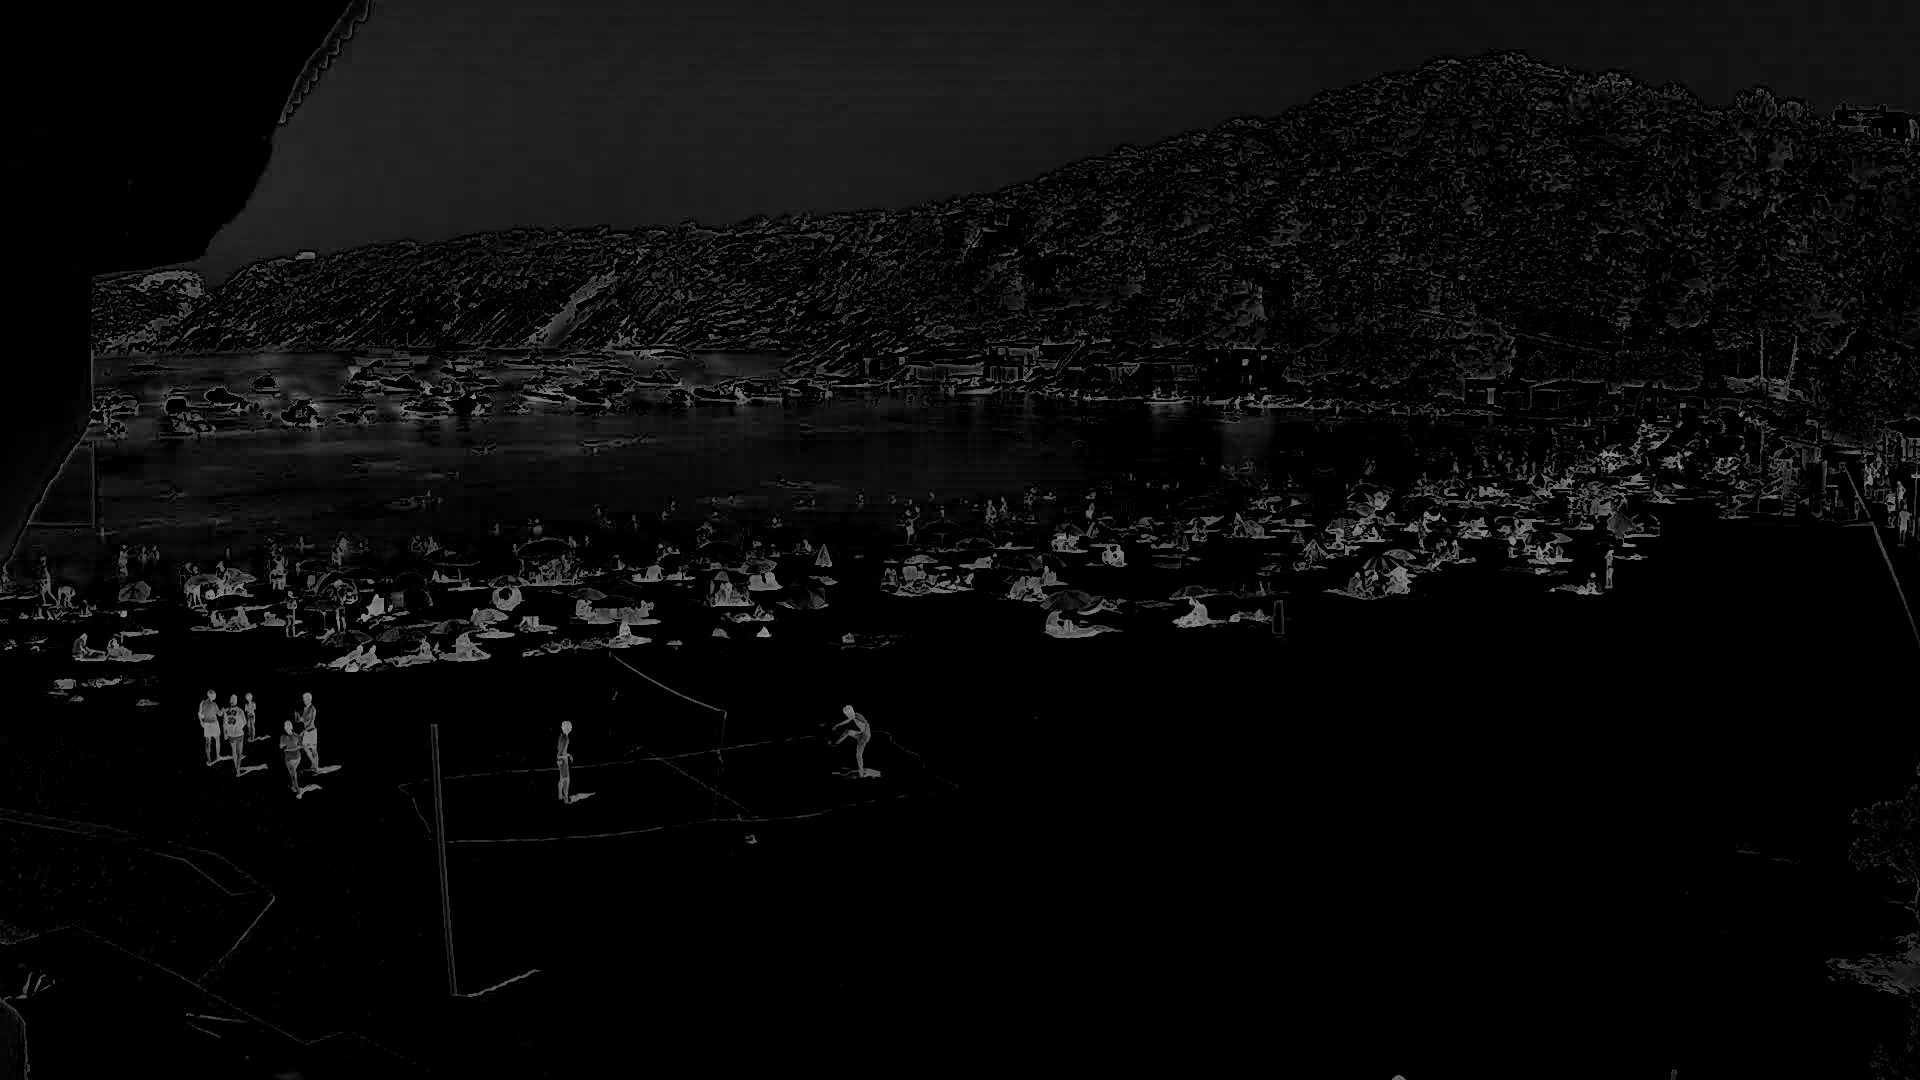
\includegraphics[width=\textwidth]{../gen/sub/1660305600.jpg}
    \end{figure}
\end{frame}

\section{Binarization}
\begin{frame}
    \frametitle{Binarization}
    \begin{figure}
        \centering
        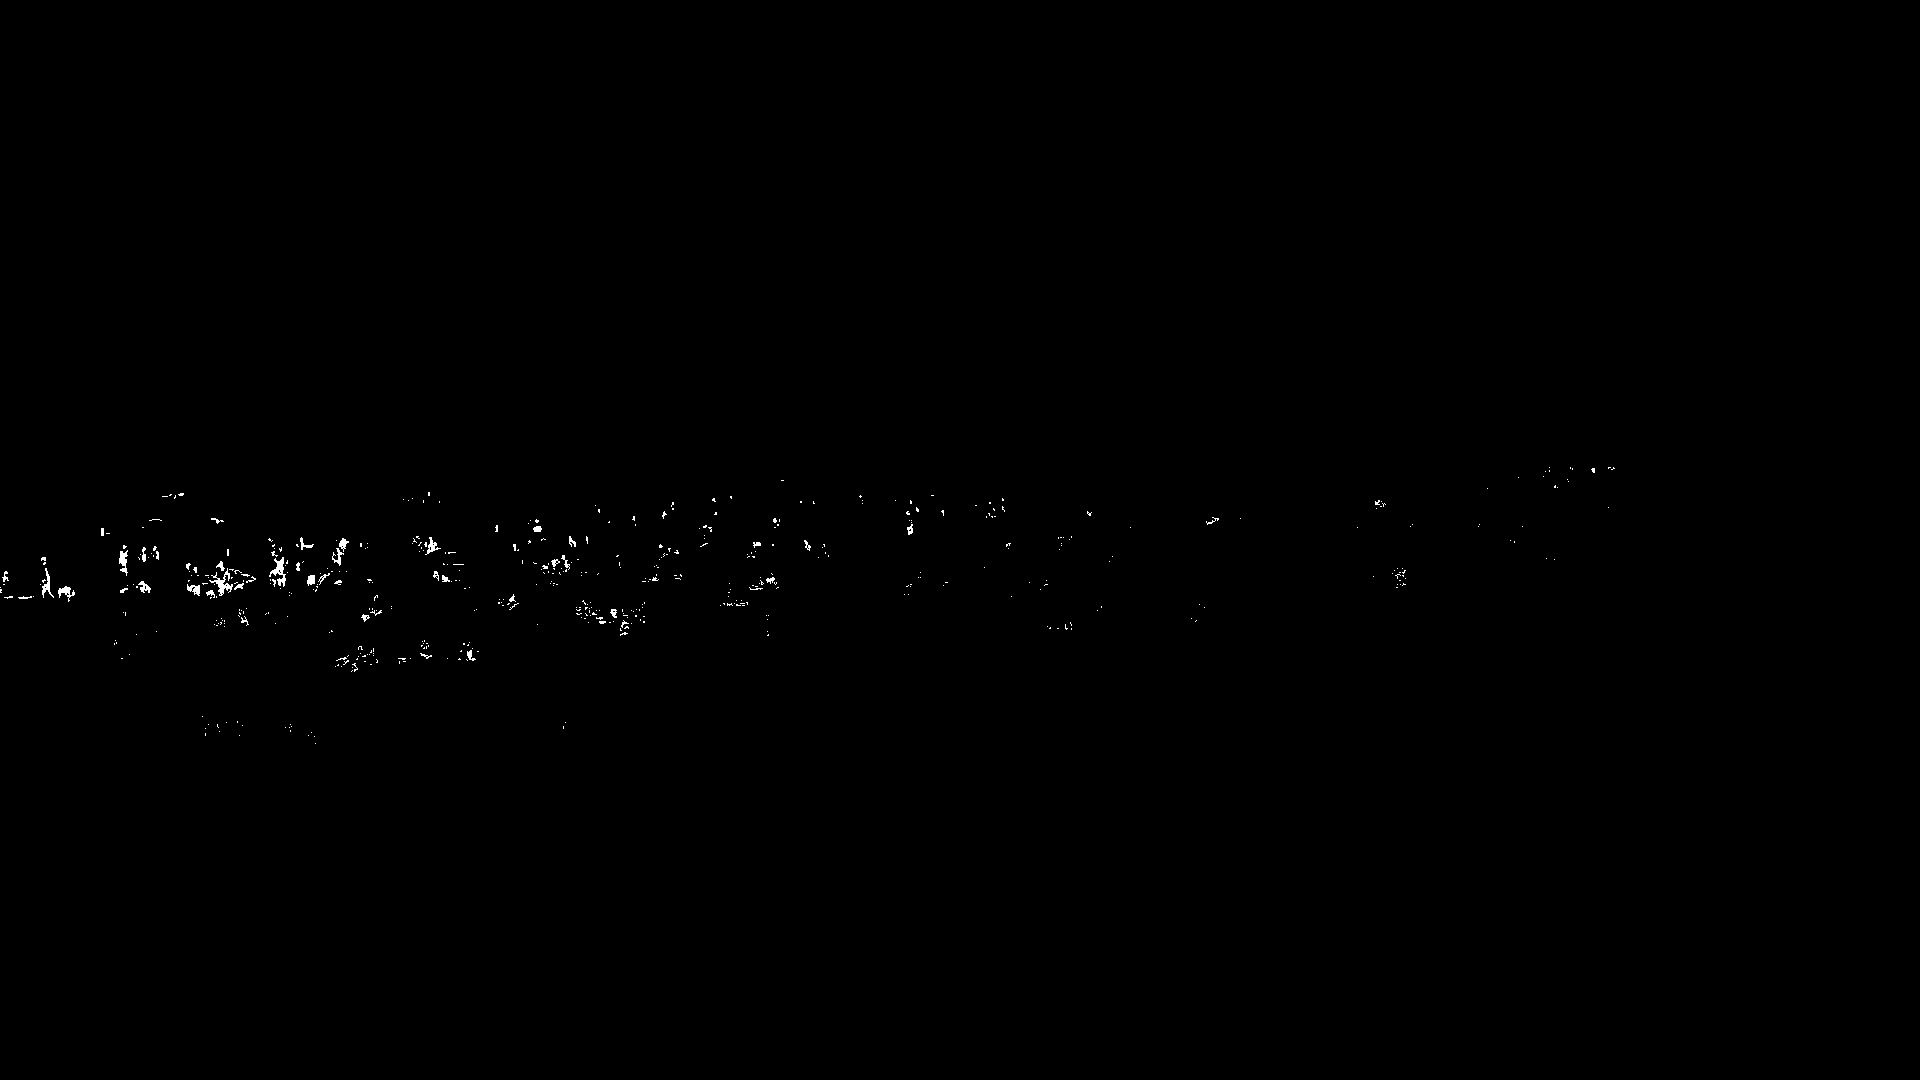
\includegraphics[width=\textwidth]{../gen/bin/1660305600.jpg}
    \end{figure}
   
        cv2.threshold(substracted, 100, 255, cv2.THRESH\_BINARY)
\end{frame}

\begin{frame}
    \frametitle{OTSU \ding{55}}
    \begin{figure}
        \centering
        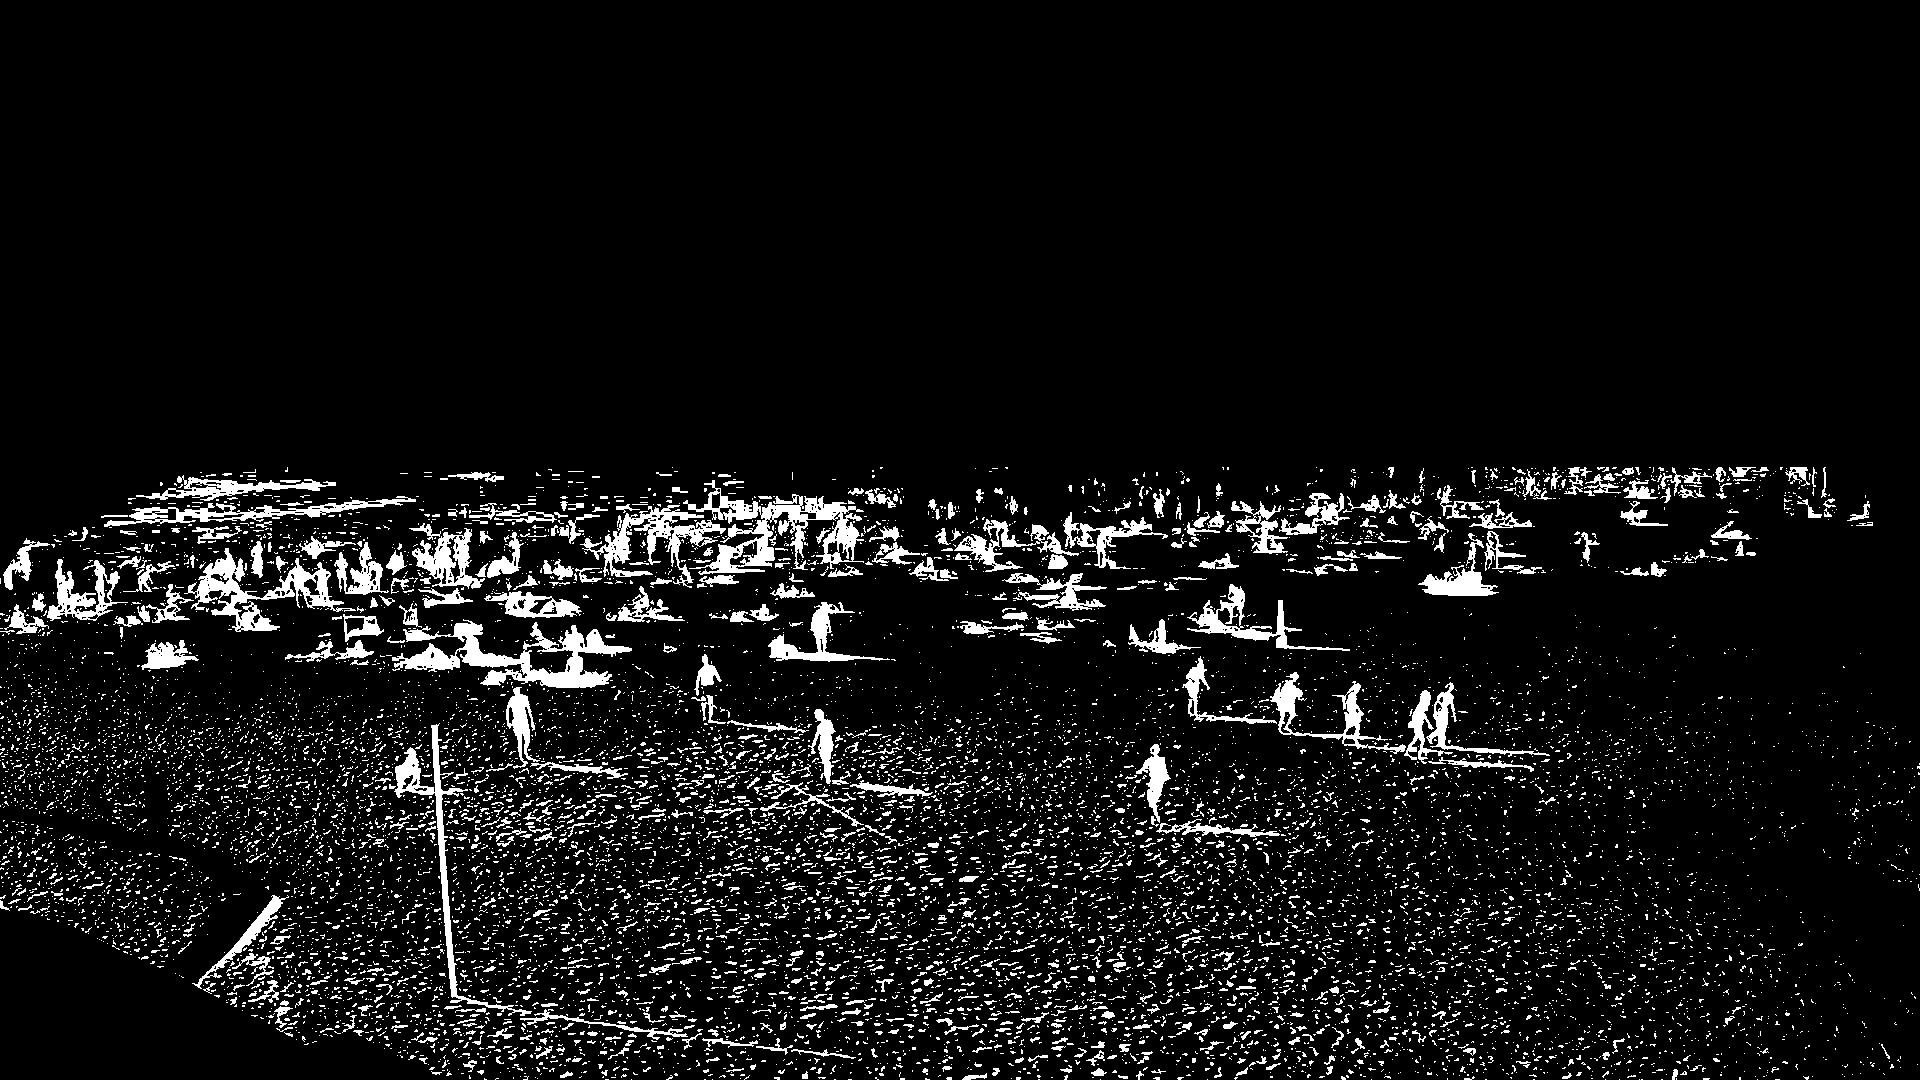
\includegraphics[width=\textwidth]{../Documentation/img/OTSU_sub_arena.jpg}
    \end{figure}
\end{frame}

\subsection*{Masking}
\begin{frame}
    \frametitle{Masking}
    \begin{figure}
        \centering
        
\includegraphics[width=\textwidth]{../mask.png}
    \end{figure}
\end{frame}

\section{Dilation}
\begin{frame}
    \frametitle{Dilation}

    \begin{figure}
        \centering
        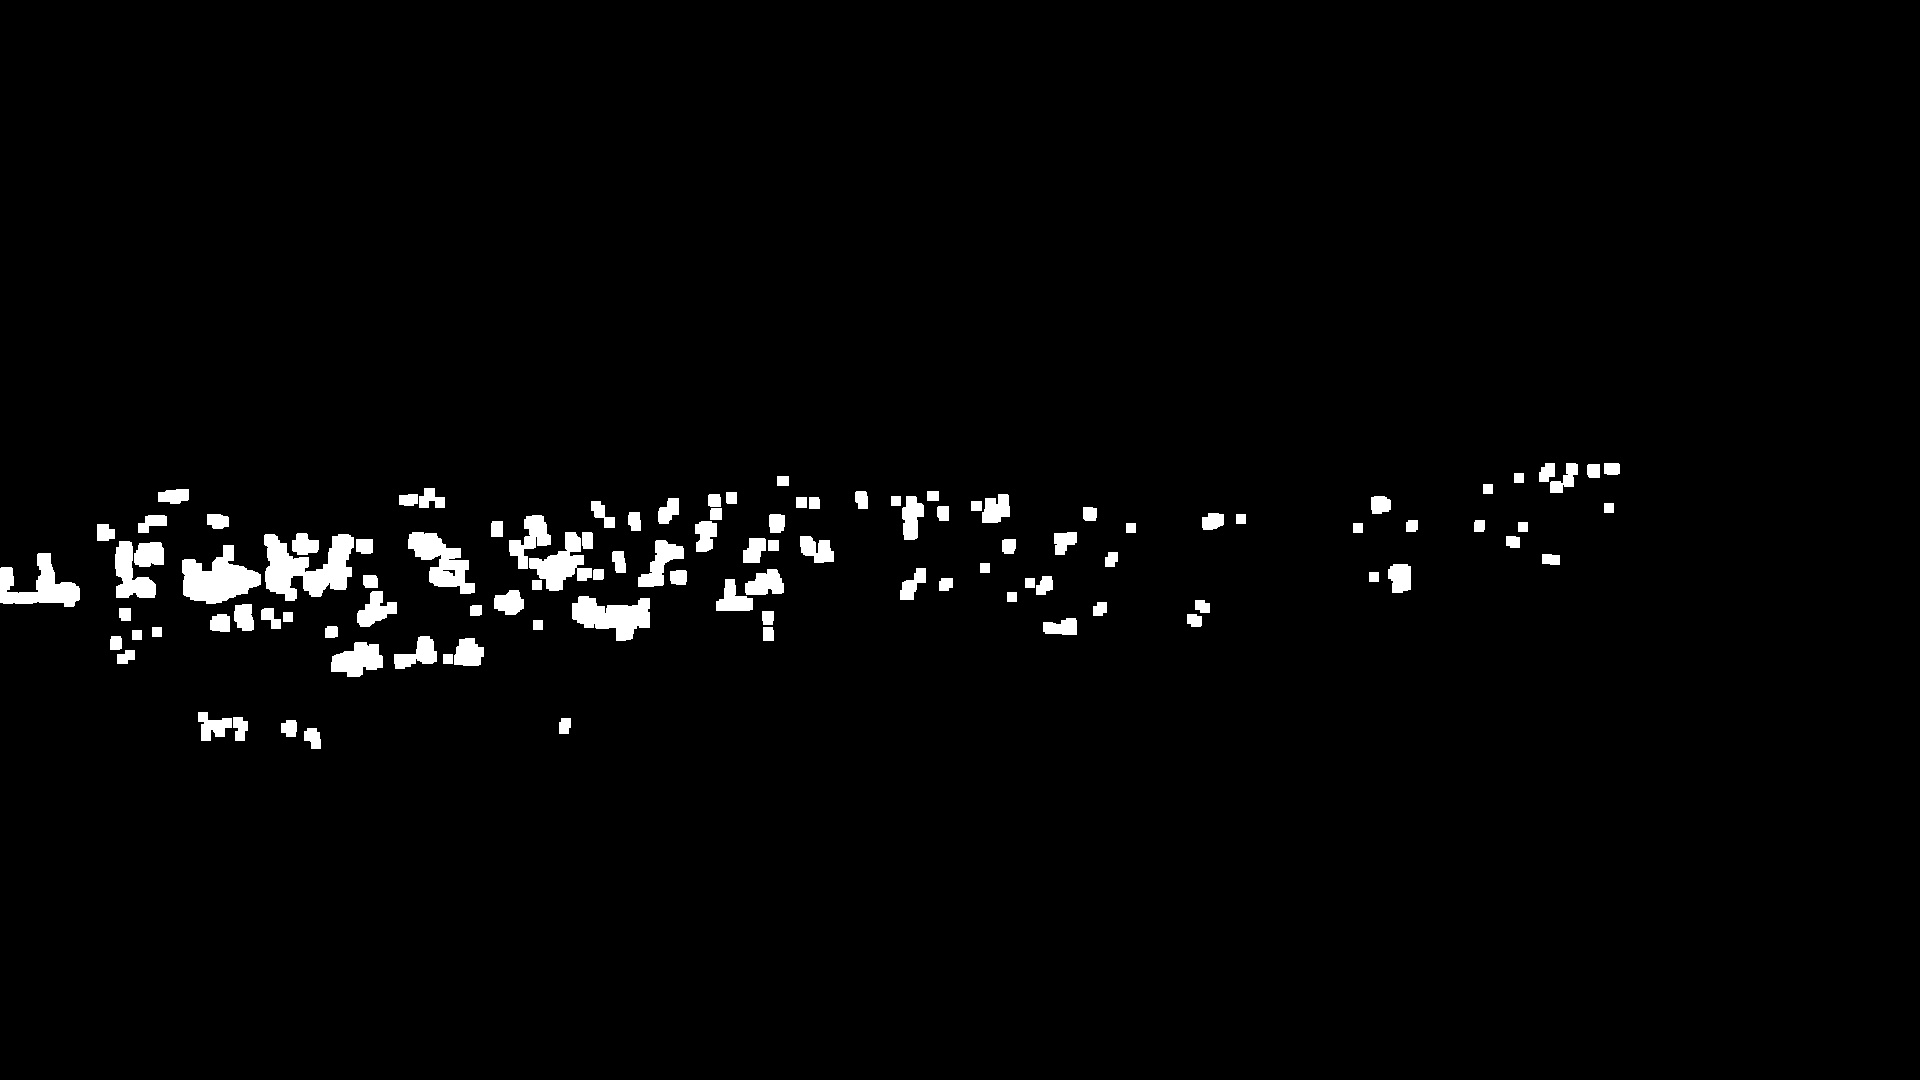
\includegraphics[width=\textwidth]{../gen/dil/1660305600.jpg}
    \end{figure}

    
\end{frame}

\section{Find contours}
\begin{frame}
    \frametitle{Find contours}
    \begin{figure}
        \centering
        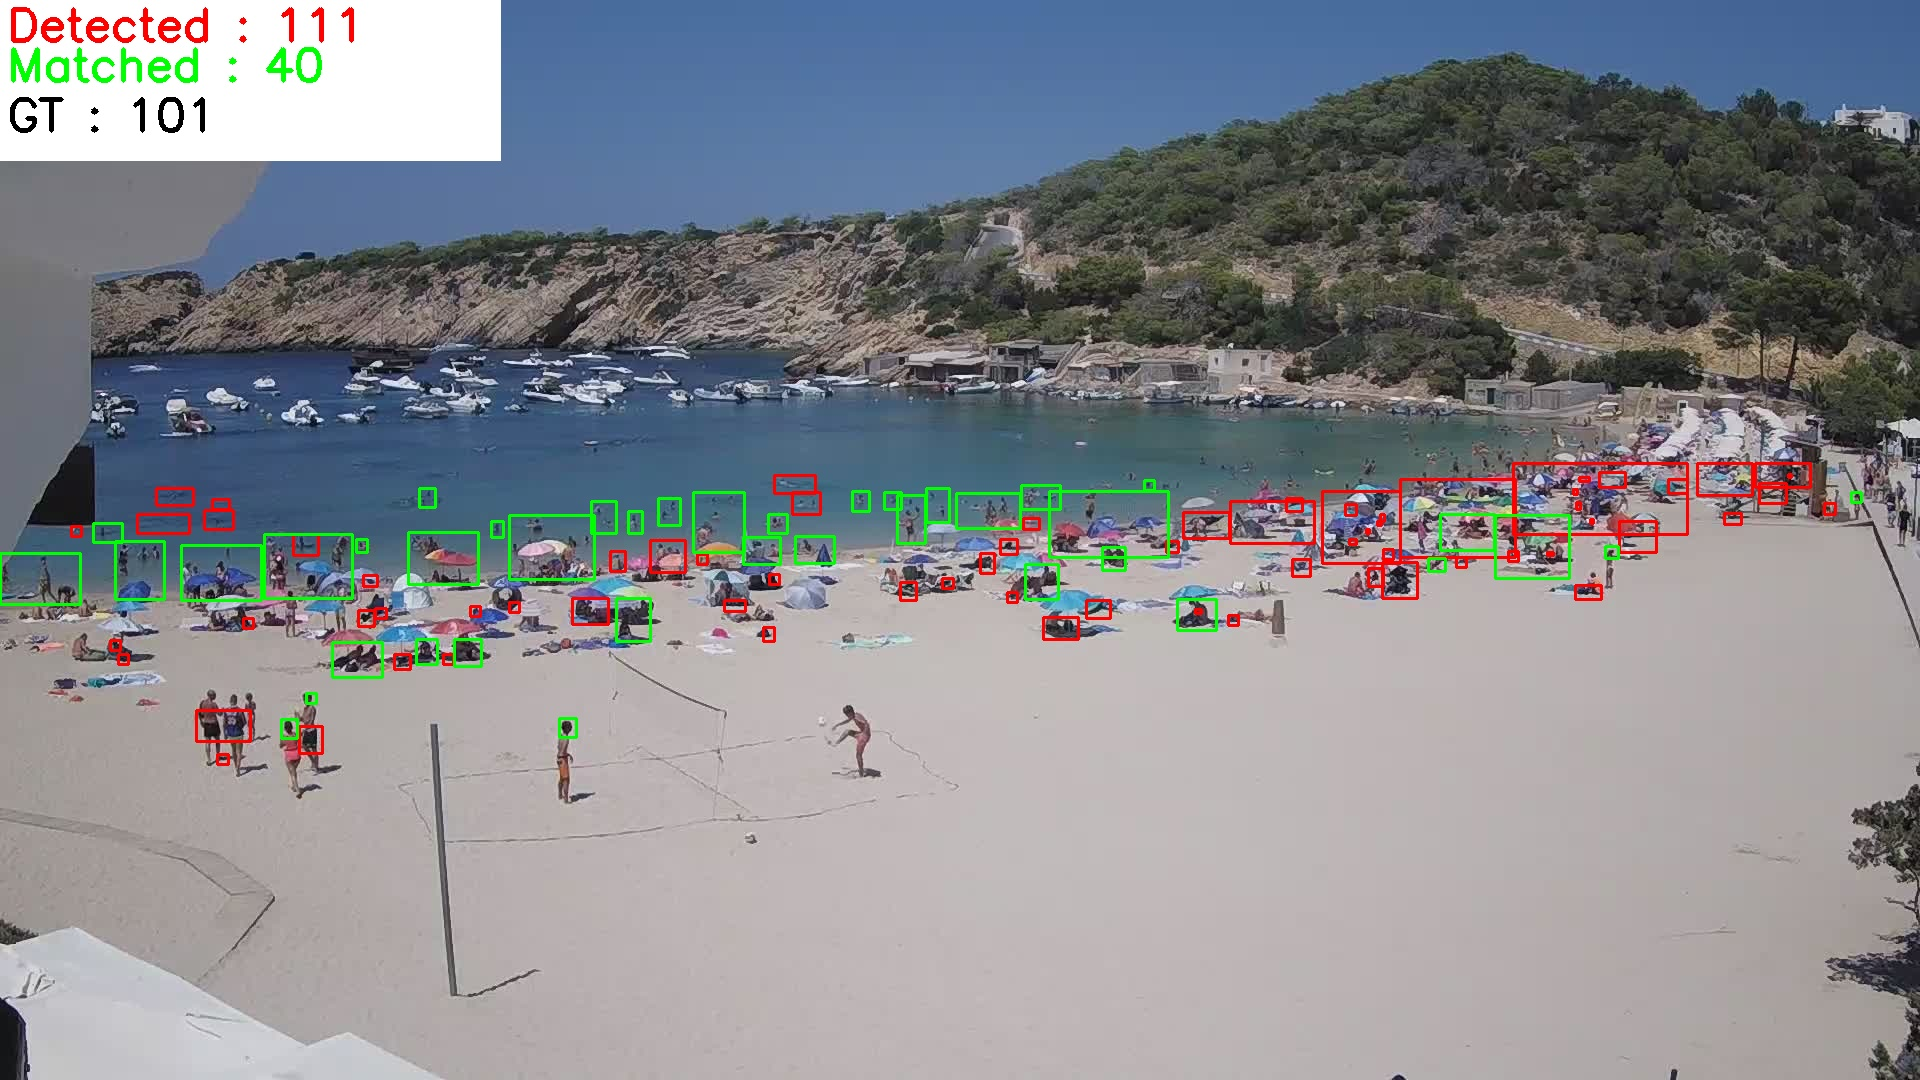
\includegraphics[width=\textwidth]{../gen/det/1660305600.jpg}
    \end{figure}
\end{frame}

%\section{Real Matching}
\begin{frame}
    \frametitle{Matching}
    \begin{figure}
        \centering
        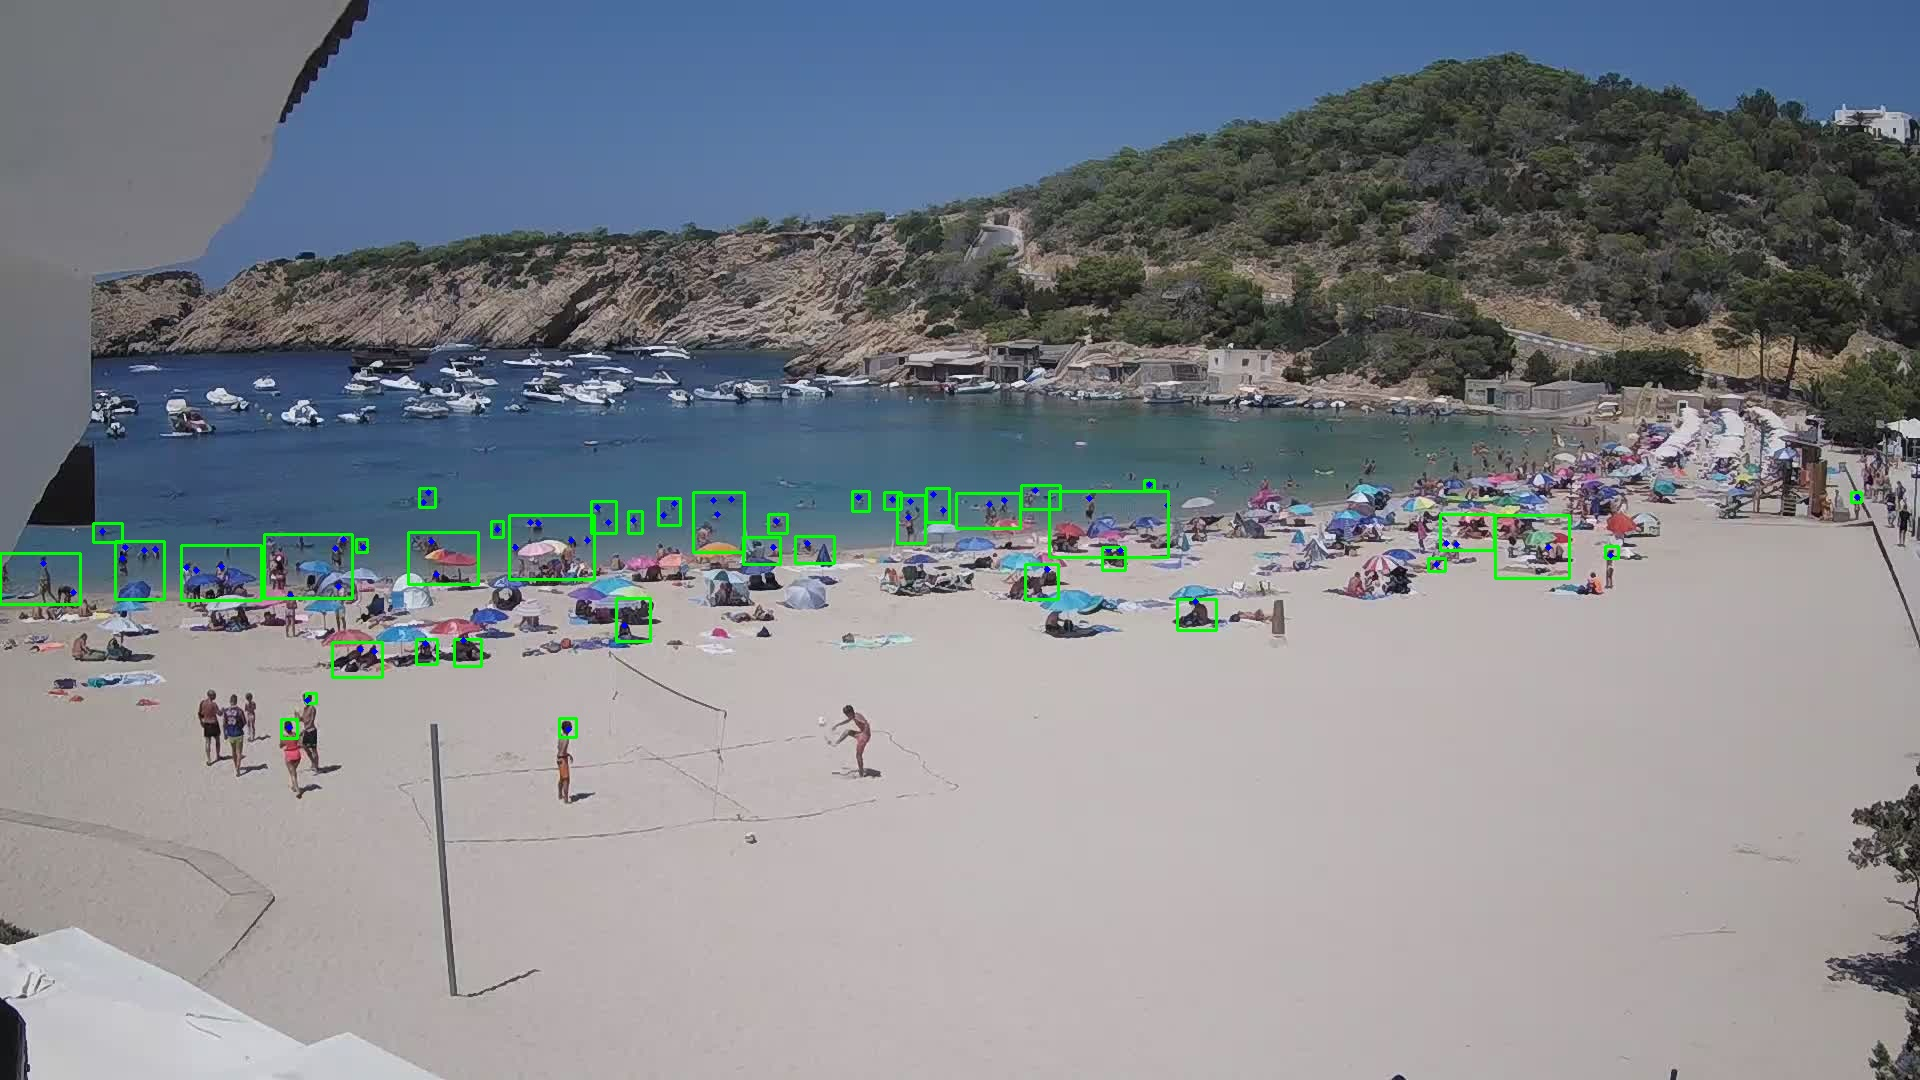
\includegraphics[width=\textwidth]{../gen/match/1660305600.jpg}
    \end{figure}
\end{frame}

\section{Results}

\begin{frame}
    \frametitle{Evaluation}
    \begin{itemize}
        
   
    \item If detection contains more than one person it will count as only one detection.
    \item In the case we would have a massive region we will discharge that detection.
    \item For checking the dimensionality of the bounding box, we would assume that width or height higher than a third of the image will not be acceptable.
    \item Regions minuscule will also be discarded.
    \item Some labels of the ground truth could be double checked.
\end{itemize}
\end{frame}

\begin{frame}
    \frametitle{Results}
    \resizebox{\textwidth}{!}{%
    %\begin{table}
        %\centering
        %\caption[Performance metrics Basic]{Performance metrics using the propossed algorithm (withouth using the empty image)}\label{table:metrics}
    \csvautobooktabular{../metrics.csv}
    %\end{table}
    }
\end{frame}

\section{Conclusions}
\begin{frame}
    \frametitle{Conclusions}
    \begin{itemize}
        \item Not seeking perfect detection.
        \item The cast shadows can confuse our algorithm.
        \item Working in color could be not ideal.
        \item The results are really fragile.
    \end{itemize}
\end{frame}






\end{document}